\documentclass[10pt]{article}

\usepackage{algorithm}
\usepackage{algpseudocode}
\usepackage{algorithmicx}
\usepackage{verbatim}

\usepackage{url}
\usepackage{xcolor}
\usepackage{natbib}
\usepackage{amsmath}
\usepackage{amssymb}
\usepackage{amsfonts}
\usepackage{graphicx}
\usepackage{verbatim}
\usepackage[top=2.5cm,bottom=2.5cm,left=2.5cm,right=2.5cm]{geometry}


\title{libcKrylov: A light weight linear solver library in C}

\author{Pengliang Yang\\
School of Mathematics, Harbin Institute of Technology, 150001, Harbin\\
E-mail: ypl.2100@gmail.com}

\begin{document}

\maketitle

\begin{abstract}

  Solution of the linear system is of fundamental importance in science and engineering applications, which can be done by direct Gaussian elimination  or iterative methods in Krylov space. We deliver a light weight library  \verb|libcKrylov| for iterative solution of linear system using C programming. The solvers include conjugate gradient (CG) method, BiCGStab and GMRES and its preconditioned variants. The construction of \verb|libcKrylov| follows the reverse communication style, allowing the system specified by a sparse banded matrix  or in a matrix-free fashion. The functionalities of the solvers are illustrated by the unsymmetric matrix inversion, and solving the large, sparse linear system after discretization of partial differential equations (the frequency domain wave equation and the Poisson equation). 

\end{abstract}

%% \begin{keyword}
%%   Linear solver \sep Krylov space \sep Partial differential equation
%% \end{keyword}


\section{Motivation and significance}

Solution of a linear system is a ubiquitous problem, thus of fundamental importance in science and engineering applications. Mathematically, it can simply be formulated as
\begin{equation}\label{eq:axb}
Ax = b,
\end{equation}
where $A \in \mathcal{C}^{m\times n}$ is a matrix of $m$ rows and $n$ columns; the vector $x\in \mathcal{C}^n$ collects all the unknowns, sometimes referred to as model parameters; $b\in \mathcal{C}^m$ is the observation vector. For a well-posed problem with $m=n$ and an invertible $A$, an intuitive and brute-force approach is direct Gauss-elimination, via lower-upper (LU) triangular matrix decomposition, whose computational complexity is of the order $O(n^3)$.  For small and medium size problem, such approaches are accurate and efficient. However, the computation and memory consumption of LU factorization easily reaches its bottleneck in 3D large-scale problems, making it infeasible to deal with practical issues. The solution of partial differential equations (Maxwell equation, wave equations, Navier-Stokes equations etc) represent a large class of such examples, yielding sparse and large linear systems to be inverted \citep{Saad_2003_IMS}.


Consequently, the iterative methods become nice and handy alternatives to address such difficulties. Besides the relaxation methods such as Jacobi and Gauss-Seidel iterations and its accelerated variants, most of the effective iterative methods are working in Krylov space. This motivates the development of \verb|libcKrylov| toolbox.
In connection to the functionalities of \verb|libcKrylov|, a number of well known computing packages such as PETSc \citep{petsc-efficient} and Trilinos \citep{heroux2005overview}  have been developed which  includes all kinds of linear solvers to deal with all kinds of computational challenges in numerical analysis. 
Let us point out that \verb|libcKrylov| is never to be new to fulfill the same goal. When developing codes for a number of interesting geophysical applications such as seismic and electromagnetic modelling and inversion, the numerical modelling are often task independent so frequent data communications and sophisticated parallelism are seldomly used.  \verb|libcKrylov| finds a niche to avoid heavy dependency of our code on a number of other irrelevant software packages that PETSc must install. The rigid syntax requirement used by Krylov solver such as PETSc can be avoided in our own applications with \verb|libcKrylov|. 


\section{Software description}

\subsection{Methods}

Let us briefly review the numerical methods implemented by \verb|libcKrylov| following \cite{Saad_2003_IMS}. The key to these numerical methods in Krylov space relies on the fact that finding the $n$ unknowns from  $m$ data points in \eqref{eq:axb} is equivalent to solving a linear inverse problem. 


When the matrix $A$ is symmetric positive definite (SPD), the most favorable iterative technique for solving equation \eqref{eq:axb} is the conjugate gradient (CG) method. It is easy to shown that \eqref{eq:axb} is normal equation of the minimization objective functional
\begin{equation}
J(x) = \frac{1}{2} x^H Ax - x^H b,
\end{equation}
where $^H$ denotes complex conjugate transpose.

There are a number of other methods when the matrix $A$ is not SPD. A simple idea is to minimize the residual of the equation in least-squares sense
\begin{equation}
J(x)=\frac{1}{2}\|Ax-b\|^2.
\end{equation}
The normal equation of the above error functional, specified by first order optimality condition $\partial J/\partial x=0$, gives
\begin{equation}
A^H Ax = A^H b.
\end{equation}
This system has a SPD coefficient matrix $A^H A$ so that it can be solved again using CG iterations. Such an approach is referred to as CGNR method. A slight different view point leads to a different method coined CGNE, by replacing $x$ with $x:=A^Hy$ in equation \eqref{eq:axb} and solving for $y$
\begin{equation}
A A^H y= b,
\end{equation}
in which $A A^H$ is again an SPD matrix. Note that CGNR achieves minimal residual while CGNE achieves minimal error (defined as the error between numerical solution $x^k$ and the true solution $x^*$, which is often unknown). Both CGNR and CGNE methods squares the condition number of the coefficient matrix, thus, these methods work well when the condition number of the matrix, $cond(A)$, is not very large.


When the condition number of the linear system in \eqref{eq:axb} is very large, the other two transpose free methods, 
biconjugate gradient stabilized (BiCGStab) version \citep{van1992bicgstab,chen2016analysis} and generalized minimal residual (GMRES) \citep{Saad_1986_GMRES} methods, are often the method of choices. GMRES ensures a monotonic decreasing trend of the equation residual, as long as sufficient computater memory is available to generate new  vectors which is orthogonal to all previous projection vectors. As memory is always an important concern in solving large scale problems, a restart strategy has been adopted, which may lead to the stagnation of the residual.
BiCGStab does not guarantee the residual vector after each iterate has a decreasing norm, however, it avoids the memory overhead of GMRES method.

Given a highly ill-conditioned problem, all the above algorithms may fail to converge within reasonable number of iterations. In such cases, a preconditioner must be designed to reach convergence. Even if the system is not close to singular, a good choice of preconditioner often makes the algorithms converge faster.

 \subsection{Software structure}

The software - \verb|libcKrylov| - consists of the following components: 
\begin{itemize}
\item \verb|src|: This folder collects all detailed implementation of many algorithms in Krylov space. These are CG, CGNE, CGNR, BiCGStab, GMRES as well as their preconditioned version. The algorithm in complex arithmetics are prefixed with a letter 'c'. A number of other algorithms such as FOM, BCG, QMR, as well as preconditioned CGNR and CGNE emthods are not included. These are important intermediate variants to more advanced algorithms such as BiCGStab and GMRES. In addition, preconditioning for CGNE and CGNR requires approximating $AA^H$ and $A^H A$, which is usually challenging and scarely used in practice.   

\item \verb|include|: There are two header files \verb|solver.h| and \verb|csolver.h|, corresponding to real (double floating point) and complex arithmetics.
  
\item \verb|lib|: This is the directory that a static library file, after compliation with 'make', will be created here, i.e., \verb|libcKrylov.a|. 
  
\item \verb|doc|: This folder contains a detailed presentation of the pseudocode associated with the algorithms implemented in \verb|src|, where a number of important references are listed. 

\item \verb|demo_poisson|, \verb|demo_wave|, and \verb|demo_toeplitz|: These are the application examples presented in the next section of this article. They should be considered as template for the use of \verb|libcKrylov|.
  
\item \verb|README.md| and \verb|LISENCE.txt|.
\end{itemize}
Figure~\ref{fig:diagram} provides a schematic diagram of \verb|libcKrylov| in a tree structure.

\begin{figure}
  \centering
  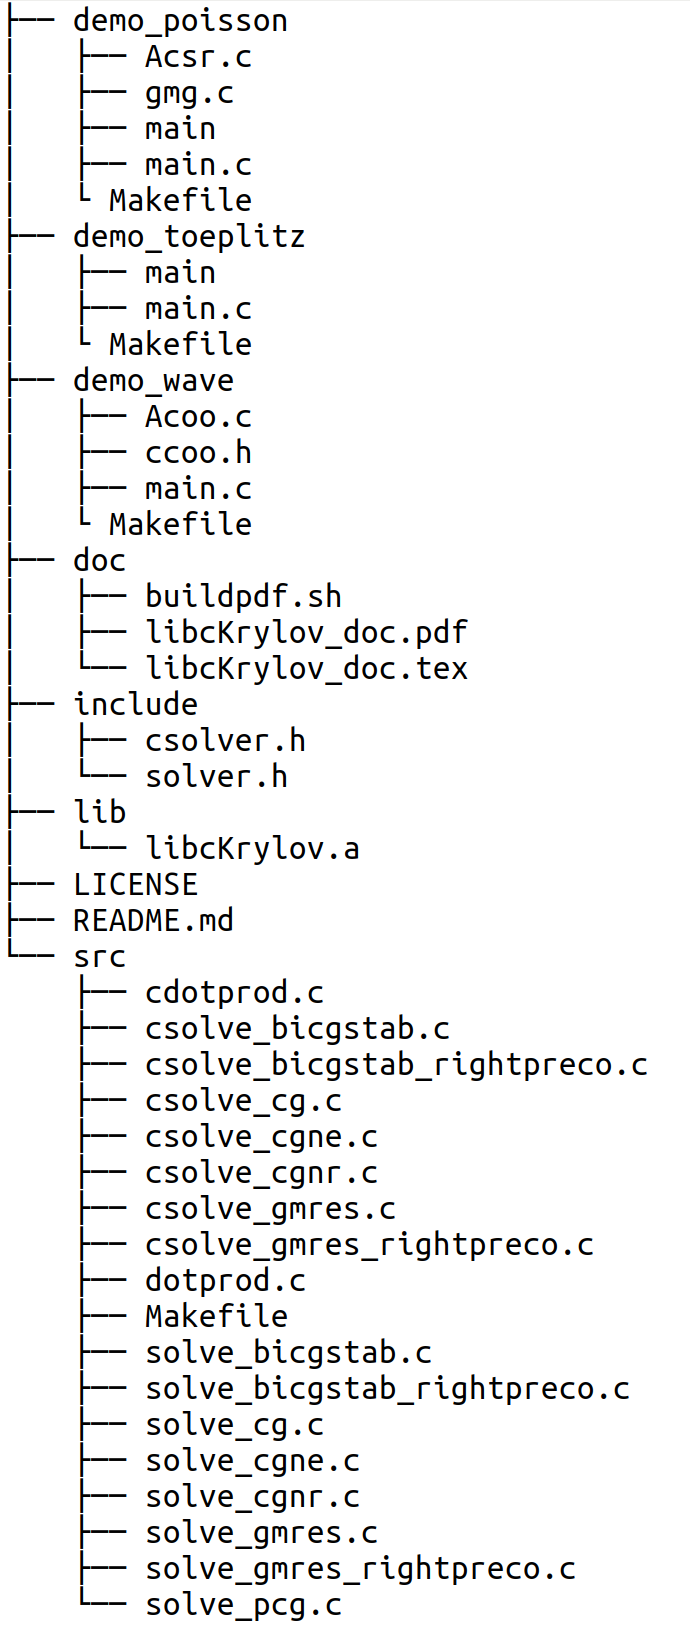
\includegraphics[width=0.5\linewidth]{list.png}\label{fig:diagram}
  \caption{The tree structure of libcKrylov}
\end{figure}


The software must be compiled with C compiler, using \verb|Makefile|. In order to use the library \verb|libcKrylov|, one must first link \verb|libcKrylov.a| when compling his/her own code by  \verb|#include "solver.h"| (or \verb|csolver.h| for complex arithmetics). Typically, consider adding the following lines in his/her own \verb|Makefile|:
\begin{verbatim} 
libcKrylov_INC = ../include
libcKrylov_LIB = ../lib

LIB = -L$(libcKrylov_LIB) -lcKrylov -lm 
INC = -I$(libcKrylov_INC) -I. 
\end{verbatim}
A good demonstration is the 'Makefile' for the 'illustrative examples'.


\subsection{Recommended coding paradigm for linear operator}

\verb|libcKrylov| toolbox can be used consistently by adding three parts of the linear solver for given problem:
\begin{itemize}
\item \verb|Aop_apply(...)| and/or possibly \verb|Atop_apply(...)|;
  We emphasis that to be consistent with all different linear solvers in \verb|libcKrylov|,  there are only 3 input parameters allowed in the linear operator, according the definition in \verb|solver.h|:
\begin{verbatim}
  typedef void (*op_t)(int, double*, double*);
\end{verbatim}
where \verb|op_t| is the placeholder for the name of the linear operator.
This means an integer \verb|n| indicating the length of the vector, the input vector \verb|x[]| and the output vector \verb|y[]| should be included in \verb|Aop_apply(n, x, y)| and \verb|Atop_apply(n, x, y)|.

\item \verb|Aop_init(...)|;
  It is clear that for most of the problems at hand, we would need a number of other important parameters. These parameters cannot be prescribed in the previous three in the linear operator. This can be done by an initialization step using \verb|Aop_init(...)|, prior to the use of \verb|Aop_apply(n, x, y)| and \verb|Atop_apply(n, x, y)|. In this step, we should allocate memory for relevant arrays, which may be visible by \verb|Aop_apply(n, x, y)| and \verb|Atop_apply(n, x, y)| internally in terms of the scope of the variables. Therefore, this function is essentially a constructor.

\item \verb|Aop_close(...)|;
  After all computations have been completed using iterative solvers, we use the routine \verb|Aop_close(...)| to free all allocated memories.   As a result, this function is essentially a destructor.
  
\end{itemize}
Note that an array allocated by \verb|Aop_init(...)| deallocated by \verb|Aop_close(...)| ensures the code is memory safe, if \verb|Aop_init| and \verb|Aop_close(...)| are called at the beginning and the end of the program.
The above three key subroutines ensure that the functionality of the linear operator is a self-contained module. Since a preconditioner, in essence, is still a linear operator, the same convention  should be adopted for coding a preconditioner. In fact, this design is no thing than the reverse communication \citep{markus2012modern} widely used by a number of Fortran codes (ARPACK for example). It is recommended to create a clean and efficient solver.


\section{Illustrative examples}

\subsection{Solution of a Toeplitz matrix system}

Our first example is the inversion of an unsymmetric Toeplitz matrix $A$, in which $A_{ij}=r_{i-j}$ corresponding to $2n-1$ different scalars $r_{-n+1},\cdots,r_0,\cdots, r_{n-1}$. Let us remark is that  we  do not need to store the whole Toeplitz matrix which is dense, but a vector $r$ with the distance between row and column indices are sufficient to represent all elements of Toeplitz matrix.
We choose $n=500$ and generate $2n-1=999$ random numbers for $r_{-n+1},\cdots r_{n-1}$. This creates an invertible matrix with relatively large condition number, allowing us to explore the performance of CGNR and CGNE methods within 200 iterations without reaching the tolerance of $10^{-6}$. Note that both the matrix and its transpose applied to a vector are required in CGNR and CGNE methods. As shown in Figure~\ref{fig:cgnrcgne}, both CGNR and CGNE have a good convergence trend. CGNR is decreasing the norm of the residual monotonically, but CGNE is not. This is consistent with the theory, as CGNE is minimizing the error between the numeric solution and the true solution, instead of minimizing the residual of the equation. 

\begin{figure}
  \centering
  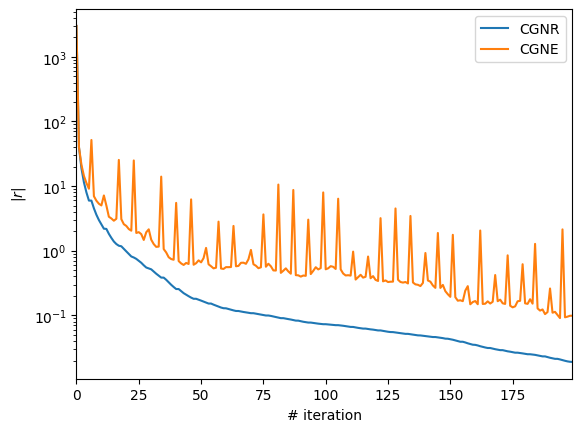
\includegraphics[width=0.7\linewidth]{cgnr_cgne.png}\label{fig:cgnrcgne}
  \caption{The convergence history of CGNR and CGNE within 200 iterations}
\end{figure}


\subsection{Frequency-domain wave equation}

The second example is to solve a frequency domain wave equation (Helmholz equation) of the following form
\begin{equation}
\left(  \frac{\partial^2}{\partial x^2} + \frac{\partial^2}{\partial z^2}\right) p(x,z,\omega) + \frac{\omega^2}{v^2(x,z)} p(x,z,\omega) = S(x,z,\omega)
\end{equation}
where $\omega$ is the angular frequency and $x,z$ are spatial coordinates, $v(x,z)$ is the wave speed, $p(x,z,\omega)$ is the pressure, $S(x,z,\omega)$ is the source term.

We discretized the wave equation using 2nd order finite difference method (hence a frequency-domain finite difference method, often coined FDFD) in space. To use truncated domain mimicking the wave propagating to infinitely far distance, we employ the perfectly matched layer (PML) technique in \citep{Hustedt_2004_MGS}. This implies that the waves are gradually attenuated in the boundary layers. The adding of PML gives a complex-valued coefficient matrix which is no more symmetric. This matrix are stored in complex numbers in triplet coordinate (COO) format \citep{barrett1994templates}.

Since the matrix is not Hermitian symmetric, we use BiCGStab and GMRES algorithms in complex arithmetics to solve the resulting linear system. Figure~\ref{fig:wave} shows the iterative solution of BiCGStab and GMRES after 100 and 300 iterations. With the increase of the number of iterations, we see that the time harmonic wave solution is expanding spatially. However, one has to pay attention to the convergence of these two algorithms in resolving Helmholz equation. According to Figure~\ref{fig:bicgstabgmres}, the GMRES with restart=10 yields a monotonic decreasing residual while BiCGStab is not. Note that both methods converges very slowly, indicating an effective preconditioner is really needed.

\begin{figure}
  \centering
  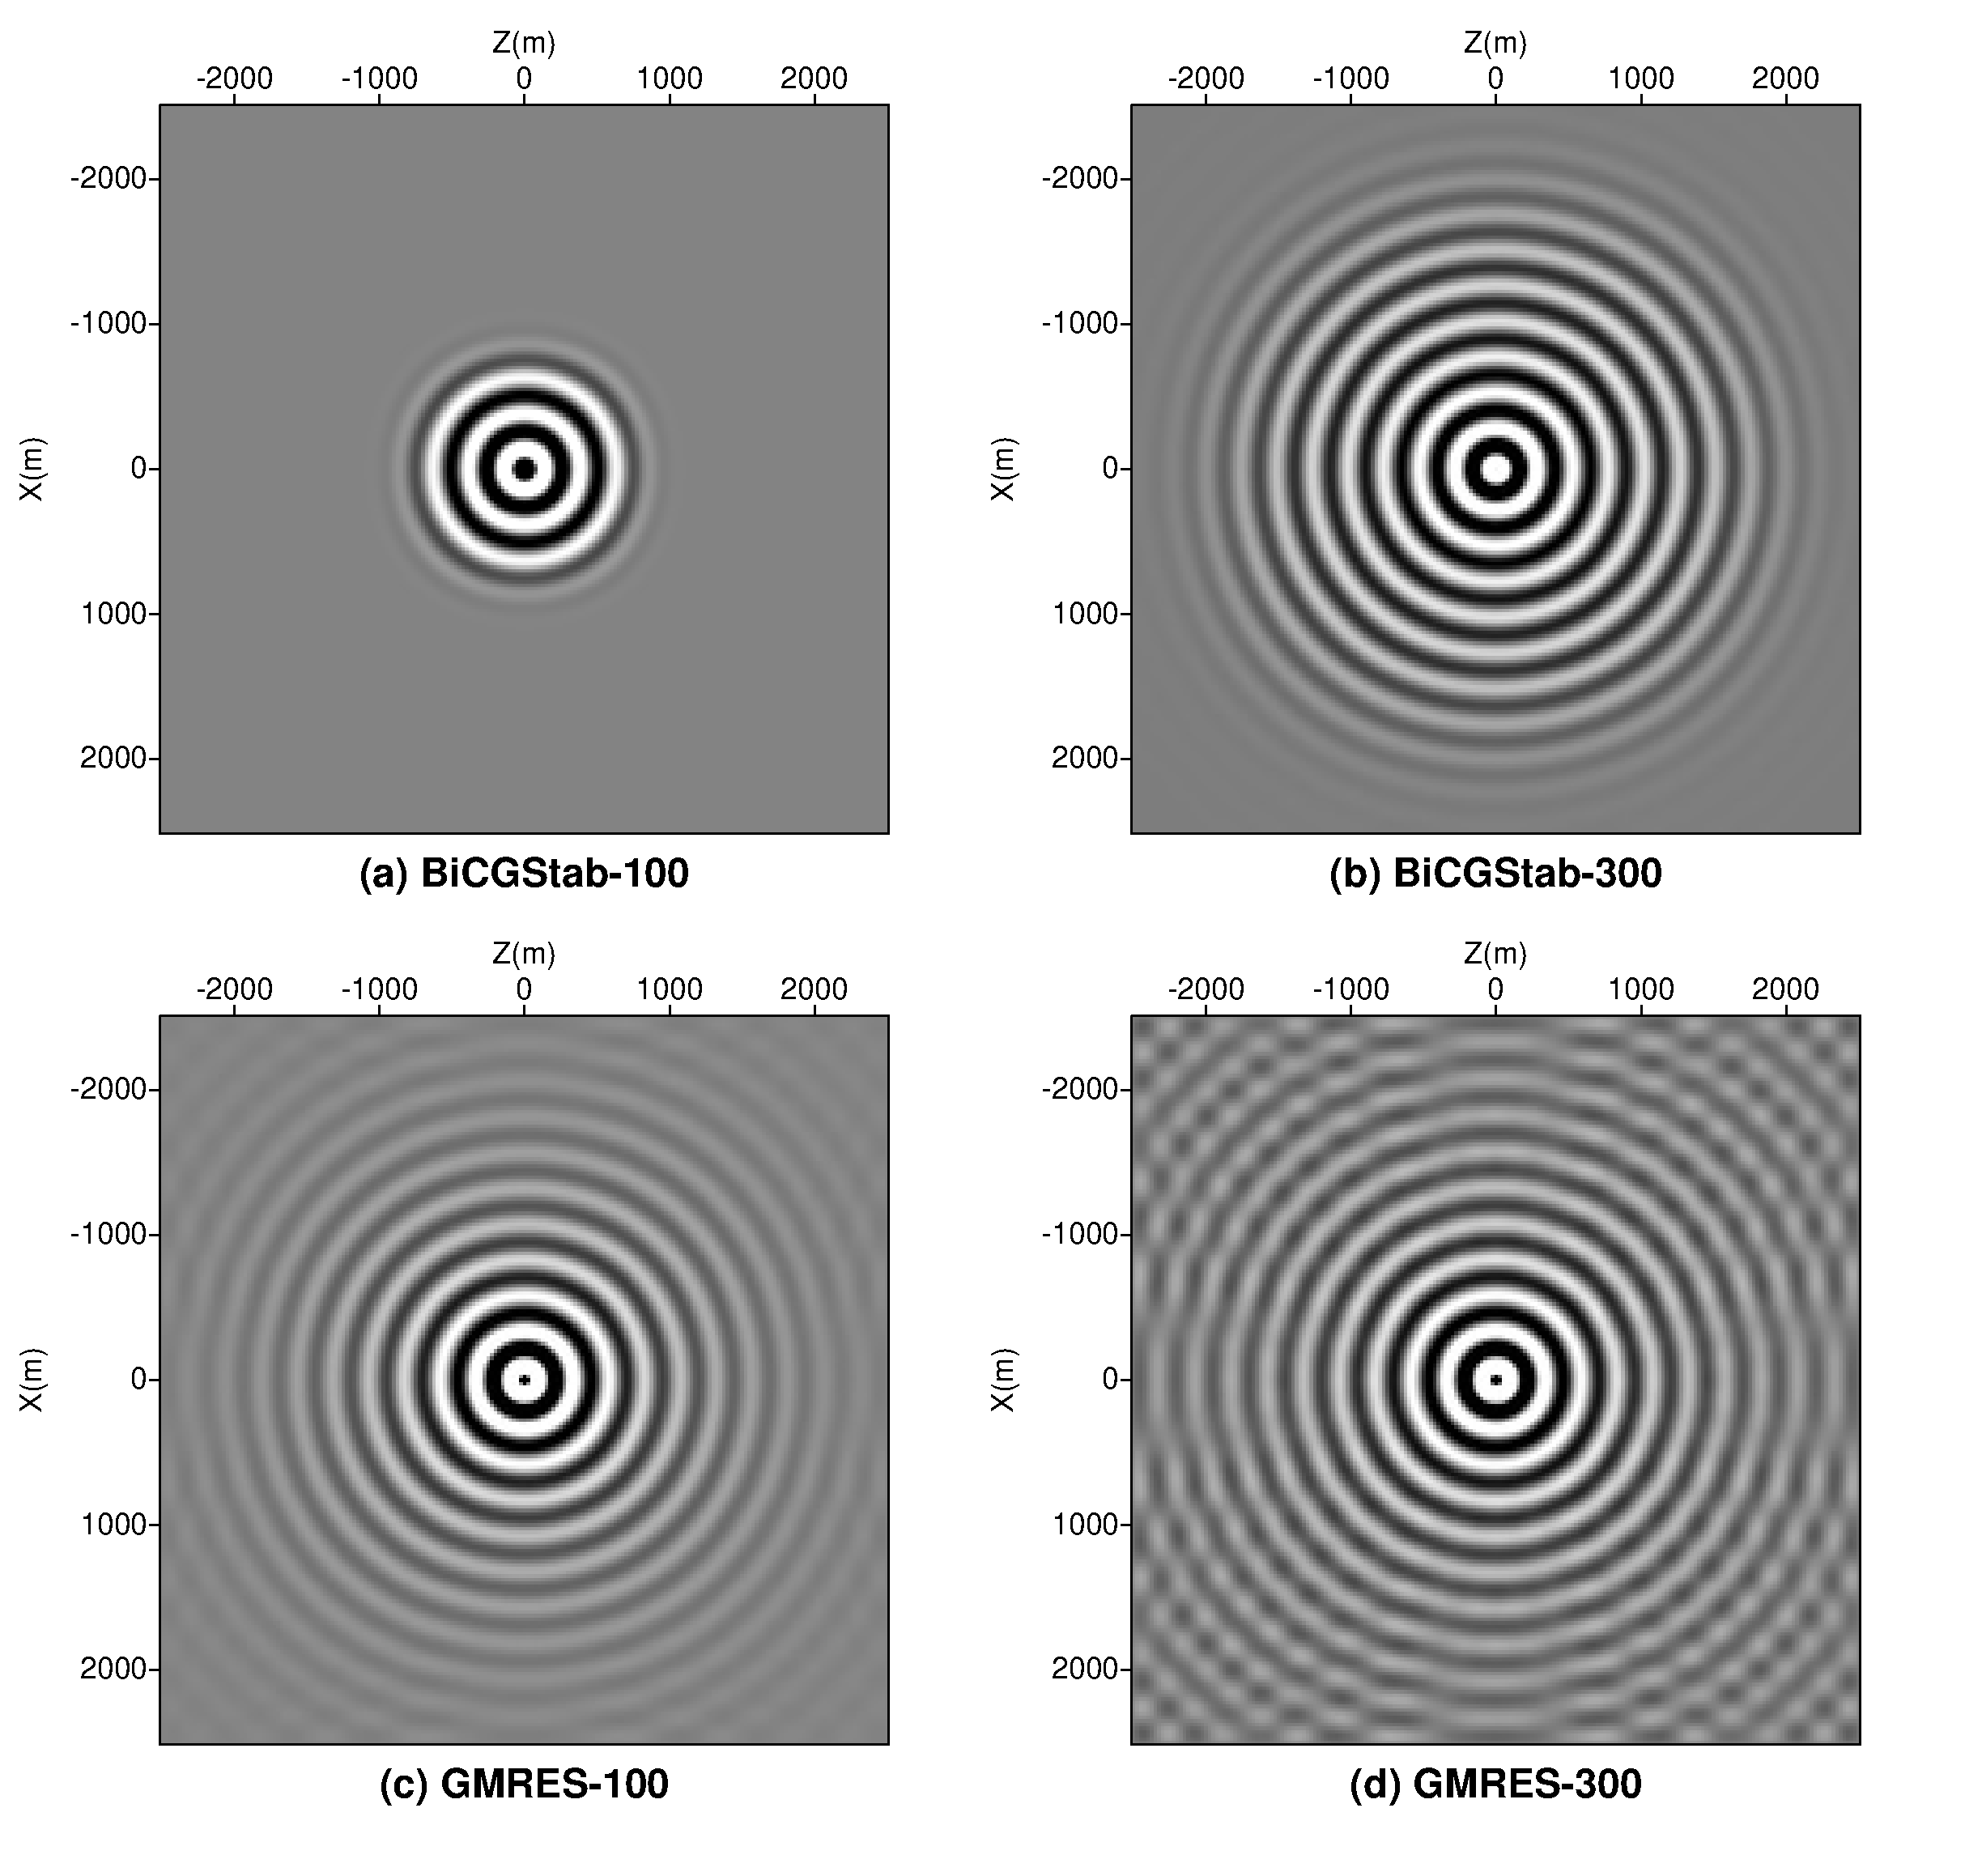
\includegraphics[width=\linewidth]{wave.pdf}\label{fig:wave}
  \caption{Frequency-domain wavefield computed by BiCGStab and GMRES (restart=10): (a) BiCGStab with 100 iterations; (b) BiCGStab with 300 iterations; (c) GMRES with 100 iterations; (d) GMRES with 300 iterations}
\end{figure}


\begin{figure}
  \centering
  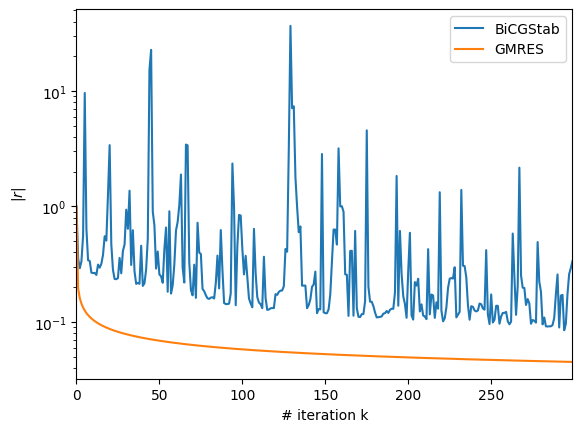
\includegraphics[width=0.7\linewidth]{bicgstab_gmres.png}\label{fig:bicgstabgmres}
  \caption{The convergence history of BiCGStab and GMRES within 300 iterations}
\end{figure}


Let us remark that solution of the wave equation is of fundamental importance in a number of geophysical applications, the problem has been continuously  pursued and still remains an active area of research. Due to prohibitive large memory requirement of direct solvers, solution of 3D wave equation using iterative solver for complex inhomogeneous models is still an open question, despite a number of interesting preconditioners have been designed \citep{Vuik_2003_SLH,Engquist_2011_SPE}. However, designing a preconditioner dedicated to Helmholtz equation is out of the scope of this software paper.


\subsection{Poisson's equation}

The third example is the Poission's equation
\begin{equation}
\left(\frac{\partial^2}{\partial x^2} + \frac{\partial^2}{\partial y^2}\right)u(x,y) = f(x,y),
\end{equation}
where we use $f(x,y) = 2(1-6x^2)y^2(1-y^2) + 2(1-6y^2)x^2(1-x^2)$. Under the homogeneous boundary condition, the analytic solution of this equation can be explicitly found: $u(x,y)=(x^2-x^4)(y^2-y^4)$, as shown in Figure~\ref{fig:poisson}a. Since the Laplacian operator is self-adjoint, it leads to a real-valued, SPD matrix system to be inverted. We store the Poisson matrix in compressed sparse row (CSR) format.
We use 200 iterations to solve the Poisson equation with a tolerence of the relative error $10^{-6}$ to test the performance of CG method and its preconditioned version using multigrid V-cycle, following \citep{Briggs_2000_Multigrid}.

Figure~\ref{fig:poisson}b and \ref{fig:poisson}c display the error between the true solution and the numeric solution found by CG and PCG. As can be seen from Figure~\ref{fig:cgpcg}, PCG converges much faster than CG: it reaches the tolerence within 58 iterations, while CG after 200 iterations still has larger errors than PCG solution. This can be obviously seen by checking the magnitude of the error panels in Figure~\ref{fig:poisson}b and \ref{fig:poisson}c. 

\begin{figure}
  \centering
  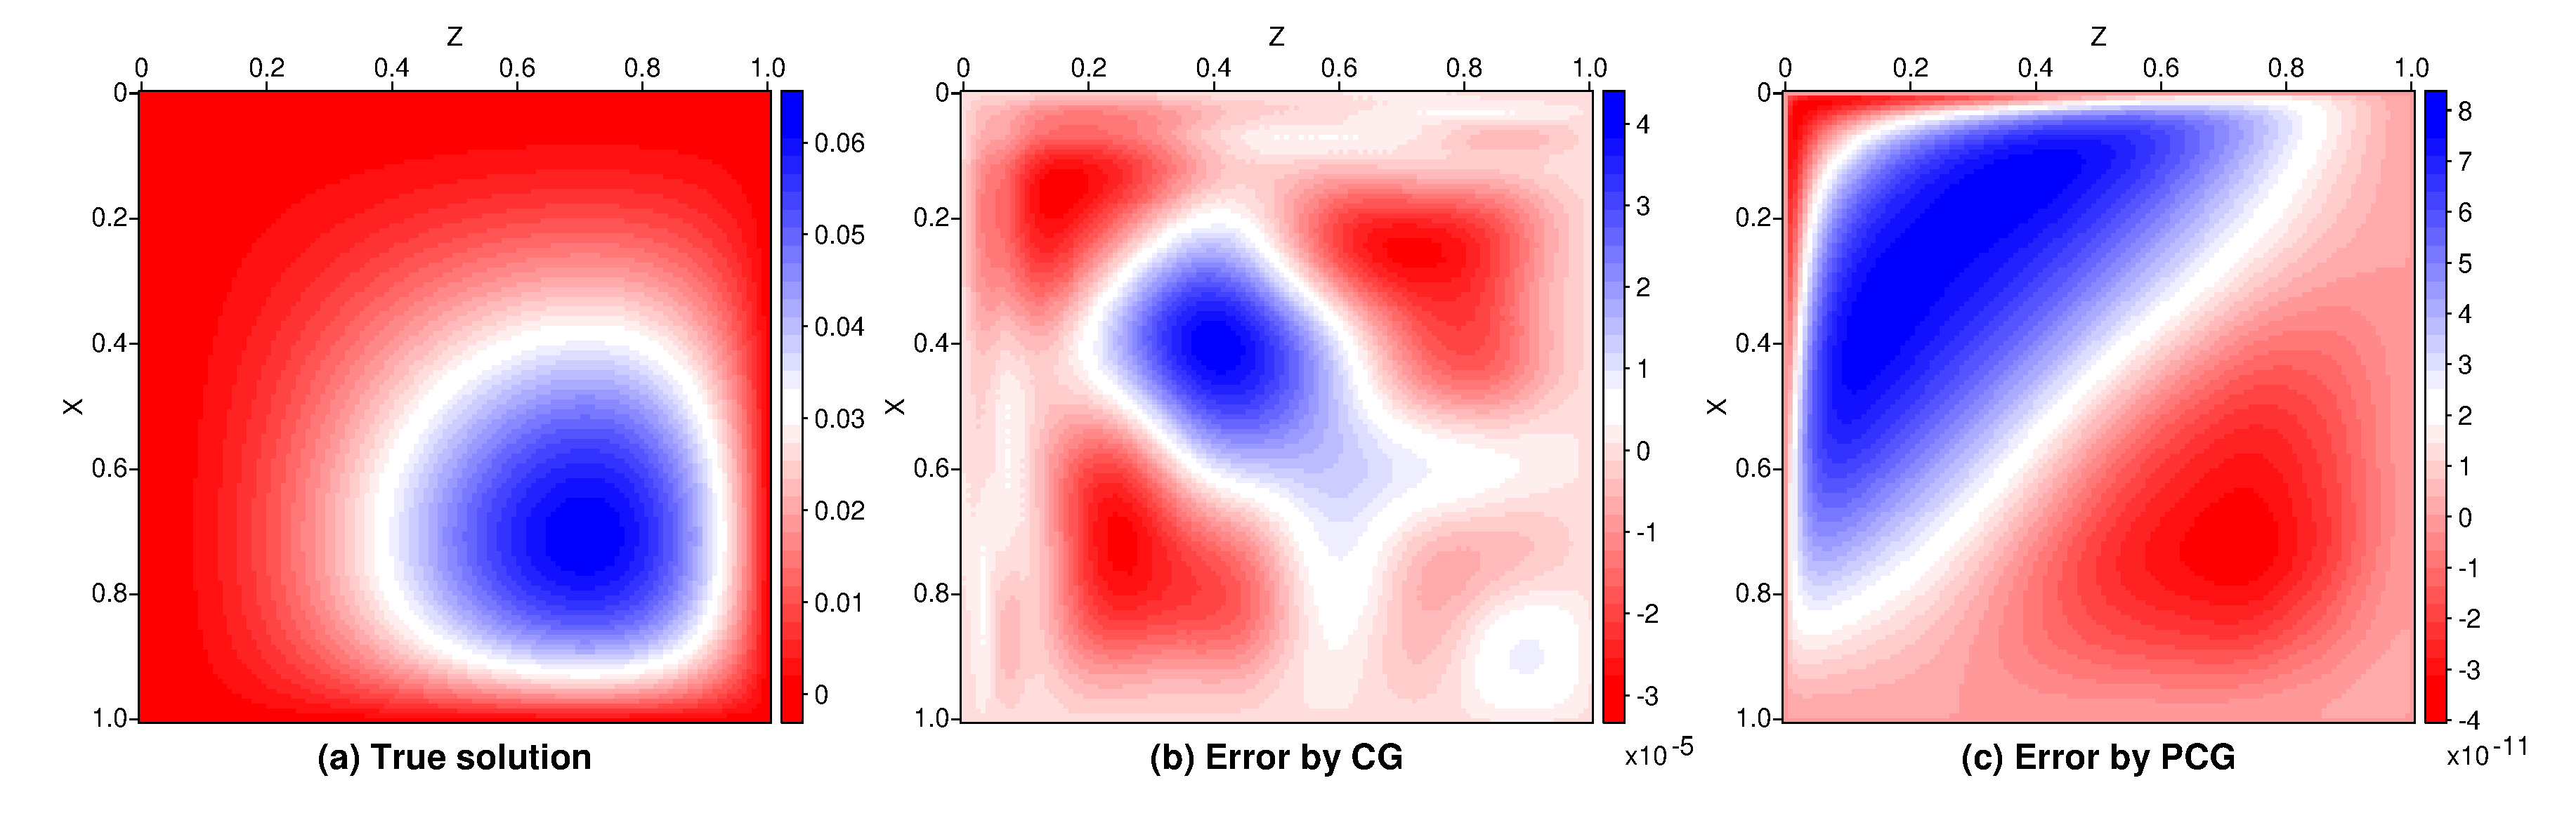
\includegraphics[width=\linewidth]{poisson.pdf}\label{fig:poisson}
  \caption{(a) The true solution $u^*$; (b) The error $|u-u^*|$ by CG; (c) The error $|u-u^*|$ by PCG.}
\end{figure}


\begin{figure}
  \centering
  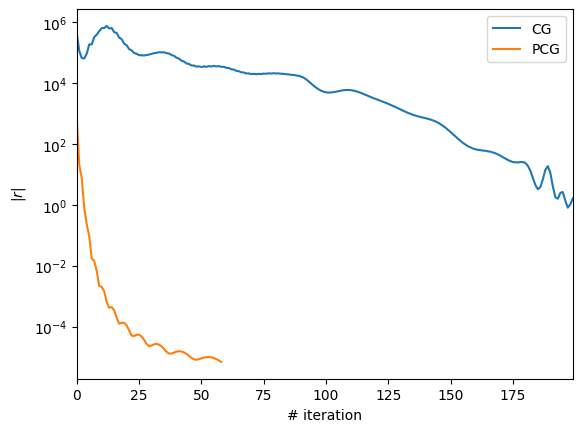
\includegraphics[width=0.7\linewidth]{cg_pcg.png}\label{fig:cgpcg}
  \caption{The convergence history of CG and PCG within 200 iterations}
\end{figure}

One thing to remark is that \verb|libcKrylov| allows a linear operator coded using compressed sparse matrix format, but also in a matrix free fasion. In this example, the geometrical multigrid preconditioner is in fact programmed in a matrix free manner, which saves the computer memory while remains efficient in implementation. On the other side, the example highlights the importance of an effective preconditioner used in iterative method to resolve the computational challenges.

\section{Conclusion}

To date, the numerical methods to solve a linear system have been well established. \verb|libcKrylov| serves as a slim and flexible code without the overhead of a number of irrelevant software packages and sophiscated data parallelism, solving the linear system using various number of Krylov space iterative methods.  Equipped with a C compiler, one can benefit from a number of mainstream linear solver, possibly combined with efficient preconditioners to address their own problem. This can be done by either linking the compiled library or directly copy relevant solver into their own project. Using \verb|libcKrylov| toolbox, one can simply focus on developing the linear operator without the need to recreate these mature solvers. 

The last two illustrative examples come from direct discretization of PDE using finite difference method, possessing a sparse banded coefficient matrix. In principle, most of the numerical methods, if not all, including finite volume method and finite element methods, lead to a large linear system, which may not necessarily be  sparse. In this case, they can still be solved with \verb|libcKrylov|: the matrix-free implementation is preferred, so that the action of the matrix applied to an input vector can be computed precisely. Based on the framework of \verb|libcKrylov| toolbox, we are currently developing a 3D least-square reverse time migration code for seismic imaging, as well as a 3D controlled-source electromagnetic modeler using preconditioned iterative approaches.

%% \section*{Declaration of competing interest}

%% I declare that I have no known competing financial interests or personal relationships that could have appeared to influence the work reported in this paper.

%% \section*{Acknowledgements}

%% The author receives the financial support from National Natural Science Fundation of China (42274156).


\section*{Code availability}

The code is accessible at github repository: \url{https://github.com/yangpl/libcKrylov}.


\appendix

\section{libcKrylov algorithm collection}

\begin{algorithm}[H]
  \caption{Conjugate gradient algorithm for solving $Ax=b$ ($A^H=A$) \citep{Shewchuk_1994_ICG}}\label{alg:CG}
  \begin{algorithmic}[1]
  \State $r_0:=b-A x_0$
  \State $p_0:=r_0$
    \For{$k=0,1,\cdots$ until convergence}
    \State $\alpha_k=\frac{r_k^H r_k}{p_k^H Ap_k}$
    \State $x_{k+1}=x_k + \alpha_k p_k$
    \State $r_{k+1}=r_k - \alpha_k A p_k$
    \State $\beta_{k} = \frac{r_{k+1}^H r_{k+1}}{r_k^H r_k}$\;
    \State $p_{k+1}=r_{k+1} + \beta_k p_k$\;
    \EndFor
  \end{algorithmic}
\end{algorithm}

\begin{algorithm}[H]
  \caption{CGNR for solving $A^H Ax=A^H b$ \citep[algorithm 8.4]{Saad_2003_IMS}}
  \begin{algorithmic}[1]
    \State $r_0=b-Ax_0$
    \State $z_0 = A^H r_0$
    \State $p_0=z_0$
    \For{$k=0,1,\cdots $ until convergence}
    \State $w_k=Ap_k$
    \State $\alpha_k = (z_k,z_k)/(w_k,w_k)$
    \State $x_{k+1} = x_k + \alpha_k  p_k$
    \State $r_{k+1} = r_k-\alpha_k w_k$
    \State $z_{k+1}=A^H r_{k+1}$
    \State $\beta_k = (z_{k+1},z_{k+1})/(z_k,z_k)$
    \State $p_{k+1}=z_{k+1}+\beta_k p_k$
    \EndFor
  \end{algorithmic}
\end{algorithm}

\begin{algorithm}[H]
  \caption{CGNE (Craig's method) for solving $AA^H y=b, x=A^H y$ \citep[algorithm 8.5]{Saad_2003_IMS}}
  \begin{algorithmic}[1]
    \State $r_0=b-Ax_0$
    \State $p_0 = A^H r_0$
    \For{$k=0,1,\cdots $ until convergence}
    \State $\alpha_k = (r_k , r_k)/(p_k, p_k )$
    \State $x_{k+1} = x_k + \alpha_k  p_k$
    \State $r_{k+1} = r_k-\alpha_k Ap_k$
    \State $\beta_k = (r_{k+1},r_{k+1})/(r_k,r_k)$
    \State $p_{k+1}=A^H r_{k+1}+\beta_k p_k$
    \EndFor
  \end{algorithmic}
\end{algorithm}

\begin{algorithm}[H]
  \caption{Preconditioned conjugate gradient algorithm for solving $Ax=b$ \citep[algorithm 9.1]{Saad_2003_IMS}}
  \begin{algorithmic}[1]
  \State $r_0:=b-A x_0=b$
  \State $z_0:=M^{-1}r_0$
  \State $p_0:=z_0$
    \For{$k=0,1,\cdots$ until convergence}
    \State $\alpha_k=\frac{r_k^H z_k}{p_k^H Ap_k}$
    \State $x_{k+1}=x_k + \alpha_k p_k$
    \State $r_{k+1}=r_k - \alpha_k A p_k$
    \State $z_{k+1}:=M^{-1}r_{k+1}$
    \State $\beta_{k} = \frac{r_{k+1}^H z_{k+1}}{r_k^H z_k}$\;
    \State $p_{k+1}=z_{k+1} + \beta_k p_k$\;
    \EndFor
  \end{algorithmic}
\end{algorithm}


\begin{algorithm}[H]
  \caption{BiCGStab \citep{chen2016analysis}, improved version from \citep{van1992bicgstab}}\label{alg:CG}
  \begin{algorithmic}[1]
    \State $r_0=b-Ax_0,$ $\tilde{r}_0$ arbitrary but $(\tilde{r}_0,r_0)\neq 0$
    \State $p_0 = r_0$
    \For{$k=0,1,\cdots $ until convergence}
    \State $\alpha_k = (r_k , \tilde{r}_0 )/(Ap_k , \tilde{r}_0 )$
    \State $s_k=r_k-\alpha_k Ap_k$ 
    \State $\omega_k = (As_k , s_k )/(As_k , As_k ) $
    \State $x_{k+1} = x_k + \alpha_k  p_k + \omega_k s_k$
    \State $r_{k+1}=s_k-\omega_k As_k$
    \State $\beta_k = (r_{k+1},\tilde{r}_0 )/(r_k,\tilde{r}_0 )\cdot \alpha_k/\omega_k$
    \State $p_{k+1}=r_{k+1}+\beta_k(p_k-\omega_k Ap_k)$
    \EndFor
  \end{algorithmic}
\end{algorithm}

\begin{algorithm}[H]
  \caption{BiCGStab with right preconditioning (Flexible BiCGStab) \citep{chen2016analysis}}\label{alg:CG}
  \begin{algorithmic}[1]
    \State $r_0=b-Ax_0,$ $\tilde{r}_0$ arbitrary but $(\tilde{r}_0,r_0)\neq 0$
    \State $p_0 = r_0$
    \For{$k=0,1,\cdots $ until convergence}
    \State $\tilde{p}_k=M^{-1}p_k$
    \State $\alpha_k = (r_k , \tilde{r}_0 )/(A\tilde{p}_k, \tilde{r}_0 )$
    \State $s_k=r_k-\alpha_k A\tilde{p}_k$
    \State $\tilde{s}_k=M^{-1}s_k$
    \State $\omega_k = (A\tilde{s}_k , s_k )/(A\tilde{s}_k,A\tilde{s}_k ) $
    \State $x_{k+1} = x_k + \alpha_k  p_k + \omega_k s_k$
    \State $r_{k+1}=s_k-\omega_k A\tilde{s}_k$
    \State $\beta_k = (r_{k+1},\tilde{r}_0 )/(r_k,\tilde{r}_0 )\cdot \alpha_k/\omega_k$
    \State $p_{k+1}=r_{k+1}+\beta_k(p_k-\omega_k A\tilde{p}_k)$
    \EndFor
  \end{algorithmic}
\end{algorithm}

Note that BICGStab above relies on inner product defined as $(x,y)=x^H y$, while GMRES below uses inner product defined as $(x,y)=x^T\bar{y}$.
\begin{algorithm}[H]
  \caption{GMRES \citep[algorithm 6.9]{Saad_2003_IMS}}
  \begin{algorithmic}[1]
    \State $r_0:=b-A x_0=b$
    \State $\beta=\|r_0\|_2$
    \State $v_1:=r_0/\beta$
    \For{$j=1,\cdots,m$}
    \State compute $w_j=Av_j$
        \For{$i=1,\cdots,j$}
        \State $h_{ij}=(w_j,v_i)$
        \State $w_j=w_j-h_{ij} v_i$
        \EndFor
    \State $h_{j+1,j}=\|w_j\|_2$. If $h_{j+1,j}=0$, set $m=j$ and go to
    \State $v_{j+1} = w_j/h_{j+1,j}$
    \State solve least-squares problem $\min_y\|\begin{bmatrix}
    \beta\\
    0\\
    \cdots\\
    0
    \end{bmatrix}- \tilde{H}_m y\|_2$ by Givens rotation
    \EndFor
    \State $x_m = x_0+V_m y_m$
  \end{algorithmic}
\end{algorithm}


\begin{algorithm}[H]
  \caption{GMRES with right preconditioning (Flexible GMRES)\citep[algorithm 9.5]{Saad_2003_IMS}}\label{alg:CG}
  \begin{algorithmic}[1]
    \State $r_0:=b-A x_0=b$
    \State $\beta=\|r_0\|_2$
    \State $v_1:=r_0/\beta$
    \For{$j=1,\cdots,m$}
    \State compute $w_j=AM^{-1}v_j$
        \For{$i=1,\cdots,j$}
        \State $h_{ij}=(w_j,v_i)$
        \State $w_j=w_j-h_{ij} v_i$
        \EndFor
    \State $h_{j+1,j}=\|w_j\|_2$. If $h_{j+1,j}=0$, set $m=j$ and go to
    \State $v_{j+1} = w_j/h_{j+1,j}$
    \State solve least-squares problem $\min_y\|\begin{bmatrix}
    \beta\\
    0\\
    \cdots\\
    0
    \end{bmatrix}- \tilde{H}_m y\|_2$ by Givens rotation
    \EndFor
    \State $x_m = x_0+M^{-1}V_m y_m$
  \end{algorithmic}
\end{algorithm}

\bibliographystyle{apalike}
%\bibliography{../biblioseiscope,../bibliopyang,../biblioothers}

\newcommand{\SortNoop}[1]{}
\begin{thebibliography}{}

\bibitem[Balay et~al., 1997]{petsc-efficient}
Balay, S., Gropp, W.~D., McInnes, L.~C., and Smith, B.~F. (1997).
\newblock Efficient management of parallelism in object oriented numerical
  software libraries.
\newblock In Arge, E., Bruaset, A.~M., and Langtangen, H.~P., editors, {\em
  Modern Software Tools in Scientific Computing}, pages 163--202.
  Birkh{\"{a}}user Press.

\bibitem[Barrett et~al., 1994]{barrett1994templates}
Barrett, R., Berry, M., Chan, T.~F., Demmel, J., Donato, J., Dongarra, J.,
  Eijkhout, V., Pozo, R., Romine, C., and Van~der Vorst, H. (1994).
\newblock {\em Templates for the solution of linear systems: building blocks
  for iterative methods}.
\newblock SIAM.

\bibitem[Briggs et~al., 2000]{Briggs_2000_Multigrid}
Briggs, W.~L., Henson, V.~E., and McCormick, S.~F. (2000).
\newblock {\em A Multigrid Tutorial, Second Edition}.
\newblock Society for Industrial and Applied Mathematics, second edition.

\bibitem[Chen et~al., 2016]{chen2016analysis}
Chen, J., McInnes, L.~C., and Zhang, H. (2016).
\newblock Analysis and practical use of flexible bicgstab.
\newblock {\em Journal of Scientific Computing}, 68(2):803--825.

\bibitem[Engquist and Ying, 2011]{Engquist_2011_SPE}
Engquist, B. and Ying, L. (2011).
\newblock Sweeping preconditioner for the {H}elmholtz equation: hierarchical
  matrix representation.
\newblock {\em Communications on pure and applied mathematics}, 64(5):697--735.

\bibitem[Heroux et~al., 2005]{heroux2005overview}
Heroux, M.~A., Bartlett, R.~A., Howle, V.~E., Hoekstra, R.~J., Hu, J.~J.,
  Kolda, T.~G., Lehoucq, R.~B., Long, K.~R., Pawlowski, R.~P., Phipps, E.~T.,
  et~al. (2005).
\newblock An overview of the trilinos project.
\newblock {\em ACM Transactions on Mathematical Software (TOMS)},
  31(3):397--423.

\bibitem[Hustedt et~al., 2004]{Hustedt_2004_MGS}
Hustedt, B., Operto, S., and Virieux, J. (2004).
\newblock Mixed-grid and staggered-grid finite difference methods for frequency
  domain acoustic wave modelling.
\newblock {\em Geophysical Journal International}, 157:1269--1296.

\bibitem[Markus, 2012]{markus2012modern}
Markus, A. (2012).
\newblock {\em Modern Fortran in practice}.
\newblock Cambridge University Press.

\bibitem[Saad, 1986]{Saad_1986_GMRES}
Saad, Y. (1986).
\newblock {GMRES}: a generalized minimal residual algorithm for solving
  nonsymmetric linear systems.
\newblock {\em {SIAM} Journal on Scientific and Statistical Computing},
  7(3):856--869.

\bibitem[Saad, 2003]{Saad_2003_IMS}
Saad, Y. (2003).
\newblock {\em Iterative {M}ethods for {S}parse {L}inear {S}ystems}.
\newblock SIAM, Philadelphia.

\bibitem[Shewchuk, 1994]{Shewchuk_1994_ICG}
Shewchuk, J.~R. (1994).
\newblock An introduction to the conjugate gradient method without the
  agonizing pain.
\newblock Technical Report Computer Science Technical Report CMU-CS-94-125,
  School of computer science, Carnegie Mellon University.

\bibitem[Van~der Vorst, 1992]{van1992bicgstab}
Van~der Vorst, H.~A. (1992).
\newblock {Bi-CGSTAB: A fast and smoothly converging variant of Bi-CG for the
  solution of nonsymmetric linear systems}.
\newblock {\em SIAM Journal on scientific and Statistical Computing},
  13(2):631--644.

\bibitem[Vuik et~al., 2003]{Vuik_2003_SLH}
Vuik, C., Erlangga, Y.~A., and Osterlee, C.~W. (2003).
\newblock Shifted laplace preconditioners for the {H}elmholtz equations.
\newblock Reports of the Departement of Applied Mathematical Analysis report
  03-18, Delft University of Technology.

\end{thebibliography}

\end{document}

